% Options for packages loaded elsewhere
\PassOptionsToPackage{unicode}{hyperref}
\PassOptionsToPackage{hyphens}{url}
\PassOptionsToPackage{dvipsnames,svgnames,x11names}{xcolor}
%
\documentclass[
  10pt,
  a4paper,
  german]{article}

\usepackage{amsmath,amssymb}
\usepackage{lmodern}
\usepackage{iftex}
\ifPDFTeX
  \usepackage[T1]{fontenc}
  \usepackage[utf8]{inputenc}
  \usepackage{textcomp} % provide euro and other symbols
\else % if luatex or xetex
  \usepackage{unicode-math}
  \defaultfontfeatures{Scale=MatchLowercase}
  \defaultfontfeatures[\rmfamily]{Ligatures=TeX,Scale=1}
\fi
% Use upquote if available, for straight quotes in verbatim environments
\IfFileExists{upquote.sty}{\usepackage{upquote}}{}
\IfFileExists{microtype.sty}{% use microtype if available
  \usepackage[]{microtype}
  \UseMicrotypeSet[protrusion]{basicmath} % disable protrusion for tt fonts
}{}
\makeatletter
\@ifundefined{KOMAClassName}{% if non-KOMA class
  \IfFileExists{parskip.sty}{%
    \usepackage{parskip}
  }{% else
    \setlength{\parindent}{0pt}
    \setlength{\parskip}{6pt plus 2pt minus 1pt}}
}{% if KOMA class
  \KOMAoptions{parskip=half}}
\makeatother
\usepackage{xcolor}
\usepackage[top=25mm,bottom=25mm,left=15mm,right=15mm]{geometry}
\usepackage[normalem]{ulem}
\setlength{\emergencystretch}{3em} % prevent overfull lines
\setcounter{secnumdepth}{3}
% Make \paragraph and \subparagraph free-standing
\ifx\paragraph\undefined\else
  \let\oldparagraph\paragraph
  \renewcommand{\paragraph}[1]{\oldparagraph{#1}\mbox{}}
\fi
\ifx\subparagraph\undefined\else
  \let\oldsubparagraph\subparagraph
  \renewcommand{\subparagraph}[1]{\oldsubparagraph{#1}\mbox{}}
\fi

\usepackage{color}
\usepackage{fancyvrb}
\newcommand{\VerbBar}{|}
\newcommand{\VERB}{\Verb[commandchars=\\\{\}]}
\DefineVerbatimEnvironment{Highlighting}{Verbatim}{commandchars=\\\{\}}
% Add ',fontsize=\small' for more characters per line
\newenvironment{Shaded}{}{}
\newcommand{\AlertTok}[1]{\textcolor[rgb]{1.00,0.33,0.33}{\textbf{#1}}}
\newcommand{\AnnotationTok}[1]{\textcolor[rgb]{0.42,0.45,0.49}{#1}}
\newcommand{\AttributeTok}[1]{\textcolor[rgb]{0.84,0.23,0.29}{#1}}
\newcommand{\BaseNTok}[1]{\textcolor[rgb]{0.00,0.36,0.77}{#1}}
\newcommand{\BuiltInTok}[1]{\textcolor[rgb]{0.84,0.23,0.29}{#1}}
\newcommand{\CharTok}[1]{\textcolor[rgb]{0.01,0.18,0.38}{#1}}
\newcommand{\CommentTok}[1]{\textcolor[rgb]{0.42,0.45,0.49}{#1}}
\newcommand{\CommentVarTok}[1]{\textcolor[rgb]{0.42,0.45,0.49}{#1}}
\newcommand{\ConstantTok}[1]{\textcolor[rgb]{0.00,0.36,0.77}{#1}}
\newcommand{\ControlFlowTok}[1]{\textcolor[rgb]{0.84,0.23,0.29}{#1}}
\newcommand{\DataTypeTok}[1]{\textcolor[rgb]{0.84,0.23,0.29}{#1}}
\newcommand{\DecValTok}[1]{\textcolor[rgb]{0.00,0.36,0.77}{#1}}
\newcommand{\DocumentationTok}[1]{\textcolor[rgb]{0.42,0.45,0.49}{#1}}
\newcommand{\ErrorTok}[1]{\textcolor[rgb]{1.00,0.33,0.33}{\underline{#1}}}
\newcommand{\ExtensionTok}[1]{\textcolor[rgb]{0.84,0.23,0.29}{\textbf{#1}}}
\newcommand{\FloatTok}[1]{\textcolor[rgb]{0.00,0.36,0.77}{#1}}
\newcommand{\FunctionTok}[1]{\textcolor[rgb]{0.44,0.26,0.76}{#1}}
\newcommand{\ImportTok}[1]{\textcolor[rgb]{0.01,0.18,0.38}{#1}}
\newcommand{\InformationTok}[1]{\textcolor[rgb]{0.42,0.45,0.49}{#1}}
\newcommand{\KeywordTok}[1]{\textcolor[rgb]{0.84,0.23,0.29}{#1}}
\newcommand{\NormalTok}[1]{\textcolor[rgb]{0.14,0.16,0.18}{#1}}
\newcommand{\OperatorTok}[1]{\textcolor[rgb]{0.14,0.16,0.18}{#1}}
\newcommand{\OtherTok}[1]{\textcolor[rgb]{0.44,0.26,0.76}{#1}}
\newcommand{\PreprocessorTok}[1]{\textcolor[rgb]{0.84,0.23,0.29}{#1}}
\newcommand{\RegionMarkerTok}[1]{\textcolor[rgb]{0.42,0.45,0.49}{#1}}
\newcommand{\SpecialCharTok}[1]{\textcolor[rgb]{0.00,0.36,0.77}{#1}}
\newcommand{\SpecialStringTok}[1]{\textcolor[rgb]{0.01,0.18,0.38}{#1}}
\newcommand{\StringTok}[1]{\textcolor[rgb]{0.01,0.18,0.38}{#1}}
\newcommand{\VariableTok}[1]{\textcolor[rgb]{0.89,0.38,0.04}{#1}}
\newcommand{\VerbatimStringTok}[1]{\textcolor[rgb]{0.01,0.18,0.38}{#1}}
\newcommand{\WarningTok}[1]{\textcolor[rgb]{1.00,0.33,0.33}{#1}}

\providecommand{\tightlist}{%
  \setlength{\itemsep}{0pt}\setlength{\parskip}{0pt}}\usepackage{longtable,booktabs,array}
\usepackage{calc} % for calculating minipage widths
% Correct order of tables after \paragraph or \subparagraph
\usepackage{etoolbox}
\makeatletter
\patchcmd\longtable{\par}{\if@noskipsec\mbox{}\fi\par}{}{}
\makeatother
% Allow footnotes in longtable head/foot
\IfFileExists{footnotehyper.sty}{\usepackage{footnotehyper}}{\usepackage{footnote}}
\makesavenoteenv{longtable}
\usepackage{graphicx}
\makeatletter
\def\maxwidth{\ifdim\Gin@nat@width>\linewidth\linewidth\else\Gin@nat@width\fi}
\def\maxheight{\ifdim\Gin@nat@height>\textheight\textheight\else\Gin@nat@height\fi}
\makeatother
% Scale images if necessary, so that they will not overflow the page
% margins by default, and it is still possible to overwrite the defaults
% using explicit options in \includegraphics[width, height, ...]{}
\setkeys{Gin}{width=\maxwidth,height=\maxheight,keepaspectratio}
% Set default figure placement to htbp
\makeatletter
\def\fps@figure{htbp}
\makeatother

\usepackage{amssymb, amsmath}
\numberwithin{equation}{section}

\usepackage[utf8]{inputenc}
\usepackage{lastpage} % counts all the pages, used in footer
\usepackage{hyperref}

% Flexible Multicolumn Option
\usepackage{multicol}
\setlength\columnsep{20pt}

% Package for enabling colors (colorful output)
\usepackage[dvipsnames]{xcolor}
\definecolor{darkgreen}{HTML}{014f32}

% Icons - http://mirrors.ctan.org/fonts/fontawesome5/doc/fontawesome5.pdf
\usepackage{fontawesome5}

% removes spacing in display math
\usepackage[nodisplayskipstretch]{setspace}

\usepackage{tabularx}

% Font Configuration
\usepackage{lmodern}
\renewcommand{\familydefault}{\sfdefault}
\usepackage{cmbright}
\usepackage[scaled=0.85]{inconsolata}

% 
\usepackage{fancyhdr}

\renewcommand{\headrulewidth}{1pt}
\renewcommand{\footrulewidth}{1pt}

\pagestyle{fancy}
\fancyhead{} % clear all header fields
\makeatletter
\fancyhead[R]{\@title\ - Zusammenfassung}
\makeatother
\fancyhead[L]{HSLU T\&A}
\fancyfoot{} % clear all footer fields
\fancyfoot[C]{\thepage\ / \pageref{LastPage}}
\fancyfoot[R]{DIDE}
\fancyfoot[L]{\today}

% introduces conditions environment to create nice equation parameter descriptions
\usepackage{array}

\newenvironment{conditions}
  {\par\vspace{\abovedisplayskip}\noindent\begin{tabular}{>{$}l<{$} @{${}:{}$} l}}
  {\end{tabular}\par\vspace{\belowdisplayskip}}
  

% Used for pandoc code block generations.
% Introduces breaklines for overflowing code blocks, by defining the Highlighting environment with breakline & symbol.
% Don't know what commandchars does :)
\usepackage{fvextra}
\DefineVerbatimEnvironment{Highlighting}{Verbatim}{
  breaklines=true,
  breakanywhere=true,
  breaksymbolleft={\textcolor{gray}{\scriptsize\ensuremath\hookrightarrow}},
  commandchars=\\\{\}
}
\makeatletter
\@ifpackageloaded{tcolorbox}{}{\usepackage[many]{tcolorbox}}
\@ifpackageloaded{fontawesome5}{}{\usepackage{fontawesome5}}
\definecolor{quarto-callout-color}{HTML}{909090}
\definecolor{quarto-callout-note-color}{HTML}{0758E5}
\definecolor{quarto-callout-important-color}{HTML}{CC1914}
\definecolor{quarto-callout-warning-color}{HTML}{EB9113}
\definecolor{quarto-callout-tip-color}{HTML}{00A047}
\definecolor{quarto-callout-caution-color}{HTML}{FC5300}
\definecolor{quarto-callout-color-frame}{HTML}{acacac}
\definecolor{quarto-callout-note-color-frame}{HTML}{4582ec}
\definecolor{quarto-callout-important-color-frame}{HTML}{d9534f}
\definecolor{quarto-callout-warning-color-frame}{HTML}{f0ad4e}
\definecolor{quarto-callout-tip-color-frame}{HTML}{02b875}
\definecolor{quarto-callout-caution-color-frame}{HTML}{fd7e14}
\makeatother
\makeatletter
\makeatother
\makeatletter
\makeatother
\makeatletter
\@ifpackageloaded{caption}{}{\usepackage{caption}}
\AtBeginDocument{%
\ifdefined\contentsname
  \renewcommand*\contentsname{Inhaltsverzeichnis}
\else
  \newcommand\contentsname{Inhaltsverzeichnis}
\fi
\ifdefined\listfigurename
  \renewcommand*\listfigurename{Abbildungsverzeichnis}
\else
  \newcommand\listfigurename{Abbildungsverzeichnis}
\fi
\ifdefined\listtablename
  \renewcommand*\listtablename{Tabellenverzeichnis}
\else
  \newcommand\listtablename{Tabellenverzeichnis}
\fi
\ifdefined\figurename
  \renewcommand*\figurename{Abbildung}
\else
  \newcommand\figurename{Abbildung}
\fi
\ifdefined\tablename
  \renewcommand*\tablename{Tabelle}
\else
  \newcommand\tablename{Tabelle}
\fi
}
\@ifpackageloaded{float}{}{\usepackage{float}}
\floatstyle{ruled}
\@ifundefined{c@chapter}{\newfloat{codelisting}{h}{lop}}{\newfloat{codelisting}{h}{lop}[chapter]}
\floatname{codelisting}{Listing}
\newcommand*\listoflistings{\listof{codelisting}{Listingverzeichnis}}
\makeatother
\makeatletter
\@ifpackageloaded{caption}{}{\usepackage{caption}}
\@ifpackageloaded{subcaption}{}{\usepackage{subcaption}}
\makeatother
\makeatletter
\@ifpackageloaded{tcolorbox}{}{\usepackage[many]{tcolorbox}}
\makeatother
\makeatletter
\@ifundefined{shadecolor}{\definecolor{shadecolor}{HTML}{f7f7f7}}
\makeatother
\makeatletter
\makeatother
\ifLuaTeX
\usepackage[bidi=basic]{babel}
\else
\usepackage[bidi=default]{babel}
\fi
\babelprovide[main,import]{ngerman}
% get rid of language-specific shorthands (see #6817):
\let\LanguageShortHands\languageshorthands
\def\languageshorthands#1{}
\ifLuaTeX
  \usepackage{selnolig}  % disable illegal ligatures
\fi
\IfFileExists{bookmark.sty}{\usepackage{bookmark}}{\usepackage{hyperref}}
\IfFileExists{xurl.sty}{\usepackage{xurl}}{} % add URL line breaks if available
\urlstyle{same} % disable monospaced font for URLs
\hypersetup{
  pdftitle={Regelungstechnik},
  pdfauthor={Joel von Rotz},
  pdflang={de},
  colorlinks=true,
  linkcolor={blue},
  filecolor={Maroon},
  citecolor={Blue},
  urlcolor={Blue},
  pdfcreator={LaTeX via pandoc}}

\title{Regelungstechnik}
\author{Joel von Rotz}
\date{14.03.23}

\begin{document}
 % [START] title
 % [ELSE] beamer

\makeatletter
\begin{center}
  \vspace*{0.5cm}
  
  \textbf{\Huge \@title}
  
  \vspace{0.1cm}
  
  \textsf{\normalsize Zusammenfassung}
  
  \vspace{0.1cm}

  {\Large {\@author \hspace{4.8cm} \@date}}
  
  \vspace{0.5cm}

\end{center}
\makeatother

 % [START] Source
\begin{center}
{\large \faGithub\space \href{https://github.com/joelvonrotz/bachelor-electrical-engineering/tree/main/semester\%204/summary/regelungstechnik}{Quelldateien}}
\end{center}
 % [END] title


 % [END] beamer
 % [END] title


% fix missing code background
\ifdefined\Shaded\renewenvironment{Shaded}{\begin{tcolorbox}[colback={shadecolor}, boxrule=0pt, frame hidden, enhanced, breakable]}{\end{tcolorbox}}\fi\ifdefined\Shaded\renewenvironment{Shaded}{\begin{tcolorbox}[frame hidden, boxrule=0pt, enhanced, breakable, colback={shadecolor}]}{\end{tcolorbox}}\fi

\renewcommand*\contentsname{Inhaltsverzeichnis}
{
\hypersetup{linkcolor=}
\setcounter{tocdepth}{3}
\tableofcontents
}
\newpage

% keep this to have smaller code blocks
\ifdefined\Shaded\renewenvironment{Shaded}{\begin{tcolorbox}[
  colback={shadecolor},
  boxrule=0pt,
  left=3pt,
  right=3pt,
  top=3pt,
  bottom=3pt,
  frame hidden,
  enhanced,
  breakable
]}{\end{tcolorbox}}\fi

\begin{multicols}{2}

\hypertarget{einfuxfchrung}{%
\section{Einführung}\label{einfuxfchrung}}

\hypertarget{ruxfcckkopplung}{%
\subsection{Rückkopplung}\label{ruxfcckkopplung}}

\emph{Rückkopplung} beschreibt eine Anordnung, bei welcher zwei oder
mehr dynamische Systeme Systeme untereinander so verbunden sind, dass
sie sich \uline{gegenseitig} beeinflussen.

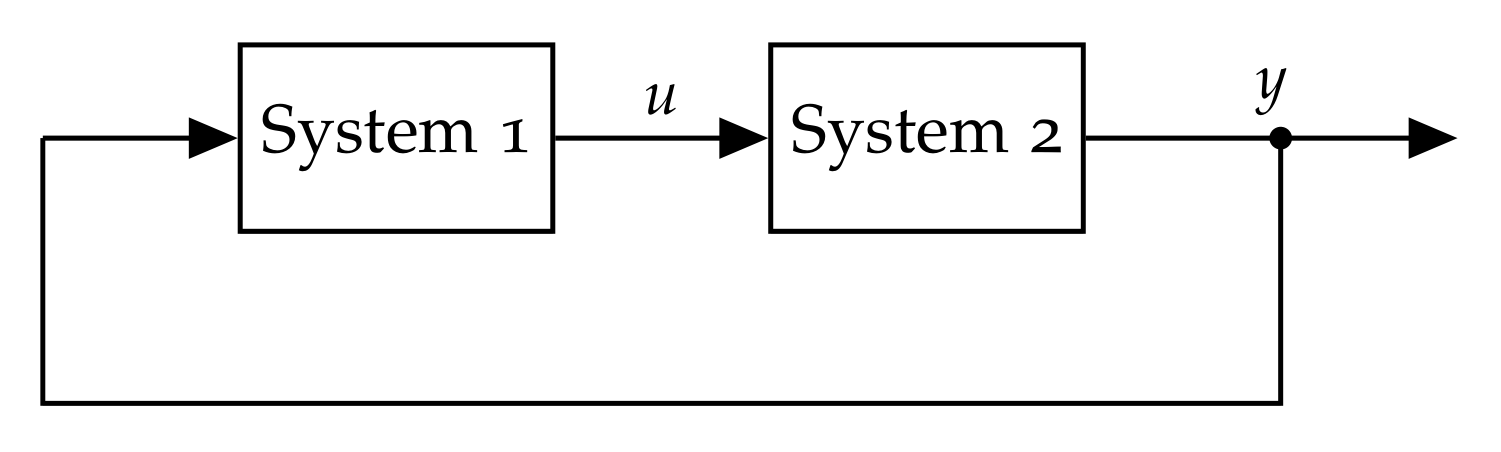
\includegraphics[width=8cm,height=\textheight]{images/closed_loop.png}

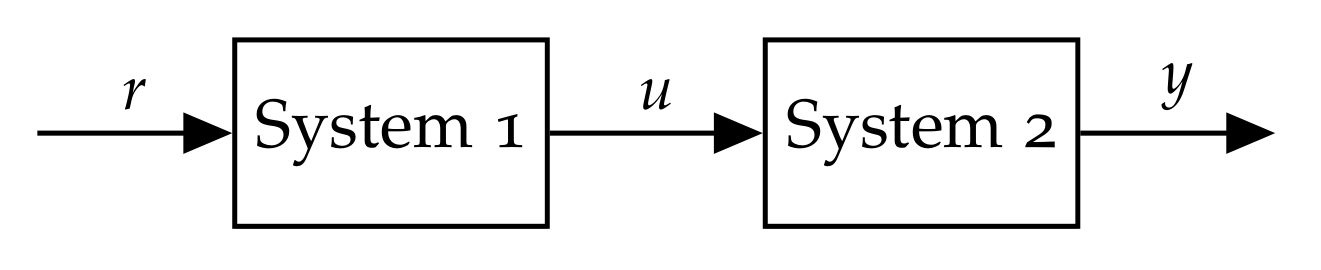
\includegraphics[width=8cm,height=\textheight]{images/open-loop.png}

Wird das Rückkopplungssignals des geschlossenen Kreises vom
Eingangssignal entfernt, also die Leitung wird aufgebrochen, wird aus
dem Kreis ein \emph{offener} Kreis.

\begin{tcolorbox}[enhanced jigsaw, bottomrule=.15mm, coltitle=black, colframe=quarto-callout-caution-color-frame, left=2mm, leftrule=.75mm, colback=white, titlerule=0mm, bottomtitle=1mm, breakable, toptitle=1mm, colbacktitle=quarto-callout-caution-color!10!white, title=\textcolor{quarto-callout-caution-color}{\faFire}\hspace{0.5em}{Vorsicht}, opacityback=0, rightrule=.15mm, arc=.35mm, opacitybacktitle=0.6, toprule=.15mm]

\textbf{Geschlossene} Kreise sind schwieriger zum Berechnen und zum
Untersuchen, da diese ein rückgekoppeltes Signal (mit dem Eingangssignal
kombinierend) Teil des Eingangssignals zum System besitzen.
\textbf{Offene} Kreise haben kein rückgekoppeltes Signal.

\end{tcolorbox}

\hypertarget{mit--und-gegenkopplung}{%
\subsection{Mit- und Gegenkopplung}\label{mit--und-gegenkopplung}}

Beide beschriebenden Systeme arbeiten nach dem Prinzip der
\emph{Gegenkopplung}

\hypertarget{steuerung-feedforward-control}{%
\subsection{\texorpdfstring{Steuerung (Feed\uline{forward}
Control)}{Steuerung (Feedforward Control)}}\label{steuerung-feedforward-control}}

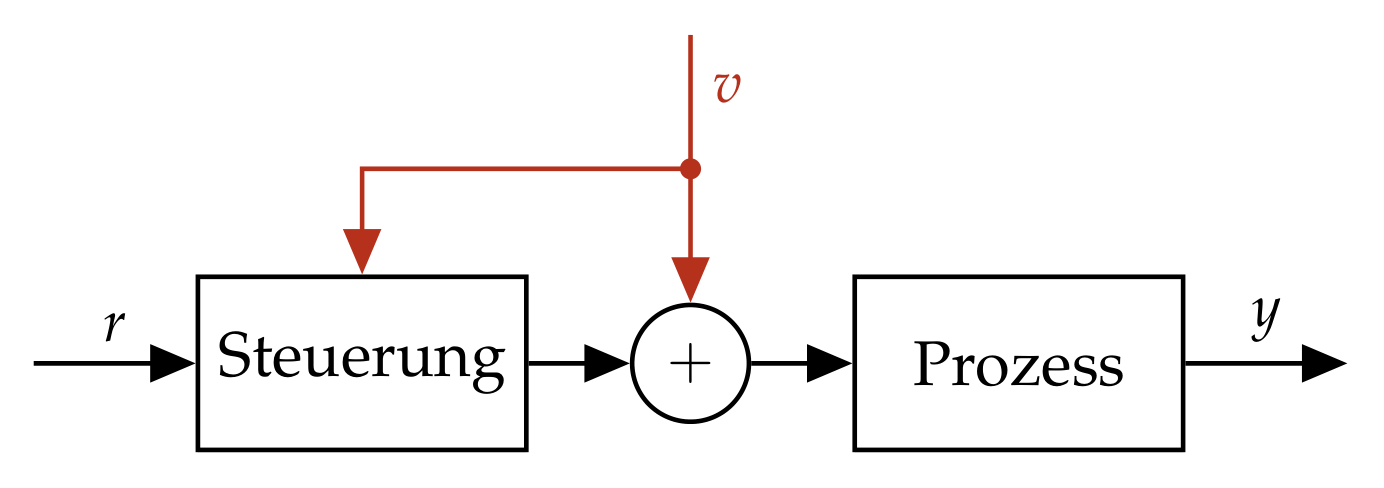
\includegraphics[width=8cm,height=\textheight]{images/steuerung.png}

\hypertarget{regelung-feedback-control}{%
\subsection{\texorpdfstring{Regelung (Feed\uline{back}
Control)}{Regelung (Feedback Control)}}\label{regelung-feedback-control}}

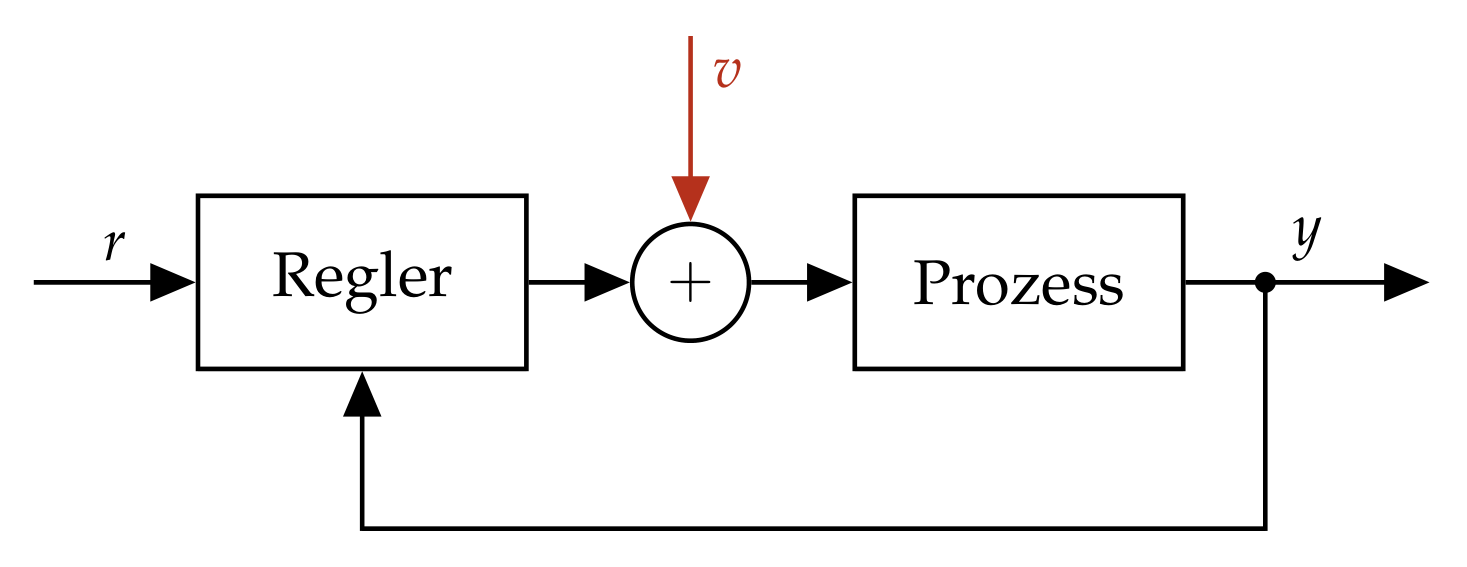
\includegraphics[width=8cm,height=\textheight]{images/regelung.png}

Ziel eines Reglers ist die Angleichung einer Regelgrösse \(y\) an eine
Führungsgrösse \(r\). Hauptmerkmal des Reglers ist die Rückkopplung und
die Fehlergrösse \(e\). Das System versucht die Fehlergrösse möglichst
auf \(0\) zu behalten, was \(r = y\) bedeutet, also die Ist-Grösse
entspricht der Soll-Grösse.

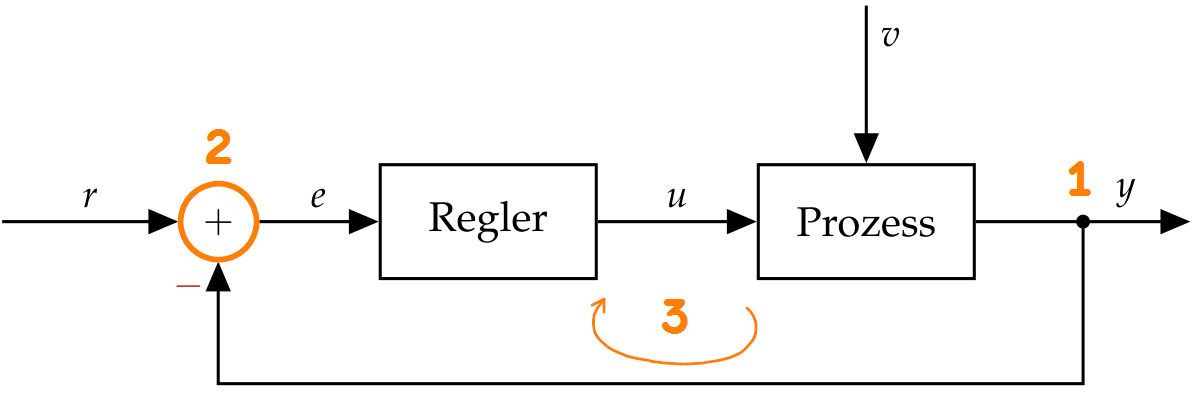
\includegraphics[width=8cm,height=\textheight]{images/definition_regelung.png}

\begin{conditions}
 r & Führungsgrösse (Soll-Wert) \\
 e & Regelfehler \\
 u & Stell-/Steuergrösse \\
 y & Regelgrösse (Ist-Wert) \\
 v & Störgrösse
\end{conditions}

\begin{tcolorbox}[enhanced jigsaw, bottomrule=.15mm, coltitle=black, colframe=quarto-callout-note-color-frame, left=2mm, leftrule=.75mm, colback=white, titlerule=0mm, bottomtitle=1mm, breakable, toptitle=1mm, colbacktitle=quarto-callout-note-color!10!white, title=\textcolor{quarto-callout-note-color}{\faInfo}\hspace{0.5em}{Merkmale einer Regelung}, opacityback=0, rightrule=.15mm, arc=.35mm, opacitybacktitle=0.6, toprule=.15mm]

Folgende Merkmale \textbf{muss} eine Regelung aufweisen. Liegt eines
nicht vor, so handelt es sich nicht um eine Regelung.

\begin{enumerate}
\def\labelenumi{\arabic{enumi}.}
\tightlist
\item
  Erfassung (Messen) der Regelgrösse
\item
  Vergleich von Regel- und Führungsgrösse
\item
  Geschlossener Wirkungskreis
\end{enumerate}

\end{tcolorbox}

\begin{align*}
y = R \cdot P \cdot e = R \cdot P\ (r-y)= R \cdot P \cdot r - R \cdot P \cdot y \\
y + R \cdot P \cdot y = R \cdot P \cdot r\quad \Rightarrow\quad\frac{y}{r}=\frac{R\cdot P}{1+R\cdot P} \stackrel{!}{=} \underline{1}
\end{align*}

\hypertarget{eigenschaften}{%
\subsubsection{Eigenschaften}\label{eigenschaften}}

\begin{itemize}
\tightlist
\item
  \textbf{Robustheit} --
\item
  \textbf{Dynamik} --
\item
  \textbf{Modularität} --
\item
  \textbf{Genauigkeit} --
\item
  \textbf{Herauserforderungen} --
\end{itemize}

\hypertarget{modellierung}{%
\section{Modellierung}\label{modellierung}}

\hypertarget{zustandsraum}{%
\subsection{Zustandsraum}\label{zustandsraum}}

\hypertarget{stuxf6rverhalten}{%
\subsection{Störverhalten}\label{stuxf6rverhalten}}

Das Störverhalten beschreibt den Einfluss der Störgrössen \(v\) auf die
Regelgrösse \(y\) bei einer konstanten Führungsgrösse \(r\). Ein gutes
Störverhalten minimiert diese Einflüsse, wobei das letzendliche
Verhalten des Systems abhängig auf das Zielsystem ist.

\uline{Beispiel}

\begin{itemize}
\tightlist
\item
  Eine Beigemaschine darf keine Überschwingungen in der Regelgrösse
  haben, da dies zu einer Überbiegung führt, was ein \emph{no-go} ist.
\item
  Eine Saune kann sich dies eher noch erlauben, da eine Überschwingung
  nur einen kleinen Einfluss auf die Systemqualität hat.
\end{itemize}

\begin{tcolorbox}[enhanced jigsaw, bottomrule=.15mm, coltitle=black, colframe=quarto-callout-note-color-frame, left=2mm, leftrule=.75mm, colback=white, titlerule=0mm, bottomtitle=1mm, breakable, toptitle=1mm, colbacktitle=quarto-callout-note-color!10!white, title=\textcolor{quarto-callout-note-color}{\faInfo}\hspace{0.5em}{Merkmale}, opacityback=0, rightrule=.15mm, arc=.35mm, opacitybacktitle=0.6, toprule=.15mm]

Die Störgrösse verfügt über vier Merkmale, welche für jedes System
betrachtet soll:

\begin{itemize}
\tightlist
\item
  \textbf{Stabilität} --
\item
  \textbf{Statischer Fehler / stationäre Genauigkeit} --
\item
  \textbf{Überschwingen} --
\item
  \textbf{Schnelles Erreichen des stationären Wertes} --
\end{itemize}

\end{tcolorbox}

\hypertarget{fuxfchrungsverhalten}{%
\subsection{Führungsverhalten}\label{fuxfchrungsverhalten}}

Das Führungsverhalten beschreibt den Einfluss der Führungs-/Sollgrösse
\(r\) auf die Regel-/Istgrösse \(y\) bei (idealerweise) einer konstanten
Störungsgrösse \(e\). Ein gutes Führungsverhalten minimiert die
Ausschwingungen und Trägheit der Regelgrösse zur Führungsgrösse.

\hypertarget{vorsteuerung}{%
\subsection{Vorsteuerung}\label{vorsteuerung}}

\hypertarget{stationuxe4ren-zustand-steady-state}{%
\subsection{Stationären Zustand (steady
state)}\label{stationuxe4ren-zustand-steady-state}}

\hypertarget{dynamik}{%
\section{Dynamik}\label{dynamik}}

\hypertarget{stabilituxe4t}{%
\subsection{Stabilität}\label{stabilituxe4t}}

Die Stabilität eines Systems wird in drei Zustände unterschieden:

\vspace{0.3cm}

\textbf{stabil}, falls alle Zustände (unterschiedliche
Anfangspositionen) in der Nähe der Gleichgewichtslage \(x_e\) zu
Lösungen führen. \textbf{asymptotisch stabil}, falls alle Zustände in
der Nähe von \(x_e\) nach langer Zeit (\(t \rightarrow \infty\)) in
\(x_e\) enden. \textbf{instabil}, falls der Zustand nie eine
Gleichgewichtslage erreicht.

\vspace{0.3cm}

\begin{tcolorbox}[enhanced jigsaw, bottomrule=.15mm, coltitle=black, colframe=quarto-callout-note-color-frame, left=2mm, leftrule=.75mm, colback=white, titlerule=0mm, bottomtitle=1mm, breakable, toptitle=1mm, colbacktitle=quarto-callout-note-color!10!white, title=\textcolor{quarto-callout-note-color}{\faInfo}\hspace{0.5em}{Beispiel}, opacityback=0, rightrule=.15mm, arc=.35mm, opacitybacktitle=0.6, toprule=.15mm]

Das Pendel, welches die gesamte Rotationsachse (\(360°\), rundherum)
ausnützen kann, hat zwei Gleichgewichtslagen. Eine Lage ist wenn die
Pendelmasse nach oben gerichtet ist und eine andere wenn die Masse nach
unten gerichtet ist.

Wird das Pendel in diese beiden Lage gelegt, ist das System
\textbf{stabil}. Wird es nach links oder nach rechts gerichtet
losgelassen, dauert es eine Weile bis es die eine Gleichgewichtslage
erreicht, dies nennt man \textbf{asymptotisch stabil}. Würde es einen
Zustand geben, wo das Pendel nie ``still steht'', nennt man dies
\textbf{instabil}.

\end{tcolorbox}

\hypertarget{linearituxe4t-zeitinvarianzen}{%
\section{Linearität \&
Zeitinvarianzen}\label{linearituxe4t-zeitinvarianzen}}

\hypertarget{adjunkte-textadja}{%
\subsection{\texorpdfstring{Adjunkte
\(\text{adj}(A)\)}{Adjunkte \textbackslash text\{adj\}(A)}}\label{adjunkte-textadja}}

\[
\text{adj}(A)=
\]

\hypertarget{lti-systeme}{%
\subsection{LTI-Systeme}\label{lti-systeme}}

\hypertarget{uxfcberlagerungsprinzip}{%
\subsubsection{Überlagerungsprinzip}\label{uxfcberlagerungsprinzip}}

\begin{tcolorbox}[enhanced jigsaw, bottomrule=.15mm, coltitle=black, colframe=quarto-callout-important-color-frame, left=2mm, leftrule=.75mm, colback=white, titlerule=0mm, bottomtitle=1mm, breakable, toptitle=1mm, colbacktitle=quarto-callout-important-color!10!white, title=\textcolor{quarto-callout-important-color}{\faExclamation}\hspace{0.5em}{Definition}, opacityback=0, rightrule=.15mm, arc=.35mm, opacitybacktitle=0.6, toprule=.15mm]

Wenn \(y_1(t)\) die Antwort auf \(u_1(t)\) ist und \(y_2(t)\) die
Antwort auf \(u_2(t)\) ist, so ist \(y_1(t) + y_2(t)\) die Antwort auf
\(u_1(t) + u_2(t)\).

\begin{figure}[H]

{\centering \includegraphics{images/überlagerungsprinzip.png}

}

\end{figure}

\end{tcolorbox}

\hypertarget{verstuxe4rkungsprinzip}{%
\subsubsection{Verstärkungsprinzip}\label{verstuxe4rkungsprinzip}}

\begin{tcolorbox}[enhanced jigsaw, bottomrule=.15mm, coltitle=black, colframe=quarto-callout-important-color-frame, left=2mm, leftrule=.75mm, colback=white, titlerule=0mm, bottomtitle=1mm, breakable, toptitle=1mm, colbacktitle=quarto-callout-important-color!10!white, title=\textcolor{quarto-callout-important-color}{\faExclamation}\hspace{0.5em}{Definition}, opacityback=0, rightrule=.15mm, arc=.35mm, opacitybacktitle=0.6, toprule=.15mm]

Wenn \(y(t)\) die Antwort auf \(u(t)\) ist, \(\alpha\cdot y(t)\) ist die
Antwort auf \(\alpha\cdot u(t)\).

\begin{figure}[H]

{\centering \includegraphics{images/verstärkungsprinzip.png}

}

\end{figure}

\end{tcolorbox}

\hypertarget{matlab}{%
\section{MATLAB}\label{matlab}}

\hypertarget{vektoren}{%
\subsection{Vektoren}\label{vektoren}}

Vektoren werden mit \texttt{{[}…{]}} deklariert. Elemente werden
Spaltenweise mit einem Leerschlag
\texttt{\textquotesingle{}\ \textquotesingle{}} oder Komma \texttt{,}
eingeteilt und mit einem Semikolon \texttt{;} Reihenweise geteilt.

\begin{Shaded}
\begin{Highlighting}[]
\VariableTok{data} \OperatorTok{=}\NormalTok{ [}\FloatTok{1}\OperatorTok{,}\FloatTok{2}\OperatorTok{,}\FloatTok{3}\OperatorTok{;}\FloatTok{4}\OperatorTok{,}\FloatTok{5}\OperatorTok{,}\FloatTok{6}\OperatorTok{;}\FloatTok{7}\OperatorTok{,}\FloatTok{8}\OperatorTok{,}\FloatTok{9}\NormalTok{]}\OperatorTok{;} \CommentTok{\% same as [1 2 3;4 5 6;7 8 9];}
\end{Highlighting}
\end{Shaded}

\begin{tcolorbox}[enhanced jigsaw, bottomrule=.15mm, coltitle=black, colframe=quarto-callout-note-color-frame, left=2mm, leftrule=.75mm, colback=white, titlerule=0mm, bottomtitle=1mm, breakable, toptitle=1mm, colbacktitle=quarto-callout-note-color!10!white, title=\textcolor{quarto-callout-note-color}{\faInfo}\hspace{0.5em}{Grösse \texttt{size}}, opacityback=0, rightrule=.15mm, arc=.35mm, opacitybacktitle=0.6, toprule=.15mm]

Mit \texttt{size} kann die Grösse einer Variable ermittelt werden.
\texttt{size} gibt als Resultat ein 1x2 Vektor zurück
(\(\begin{bmatrix}\text{Rows} & \text{Columns}\end{bmatrix}\))

\begin{Shaded}
\begin{Highlighting}[]
\OperatorTok{\textgreater{}\textgreater{}} \VariableTok{a} \OperatorTok{=} \FloatTok{1}
\OperatorTok{\textgreater{}\textgreater{}} \VariableTok{size}\NormalTok{(}\VariableTok{a}\NormalTok{)}
     \FloatTok{1}     \FloatTok{1}  \CommentTok{\% rows, columns}
\end{Highlighting}
\end{Shaded}

\end{tcolorbox}

\begin{Shaded}
\begin{Highlighting}[]
\VariableTok{a} \OperatorTok{=} \FloatTok{1}
\end{Highlighting}
\end{Shaded}

\[
\begin{bmatrix}
1
\end{bmatrix}\qquad \text{oder einfach}\qquad 1 
\]

Die \texttt{size}-Funktion gibt auch bei einzelnen Werte eine Grösse
aus, nämlich \(\begin{bmatrix}1 & 1\end{bmatrix}\)

\begin{Shaded}
\begin{Highlighting}[]
\VariableTok{b} \OperatorTok{=}\NormalTok{ [}\FloatTok{1} \FloatTok{2} \FloatTok{3}\NormalTok{] }\CommentTok{\% Linienvektor}
\end{Highlighting}
\end{Shaded}

\[
\begin{bmatrix}
1 & 2 & 3
\end{bmatrix}
\]

\begin{Shaded}
\begin{Highlighting}[]
\VariableTok{c} \OperatorTok{=}\NormalTok{ [}\FloatTok{2}\OperatorTok{;}\FloatTok{3}\OperatorTok{;}\FloatTok{4}\NormalTok{] }\CommentTok{\% Spaltenvektor}
\end{Highlighting}
\end{Shaded}

\[
\begin{bmatrix}
2 \\ 3 \\ 4
\end{bmatrix}
\]

\hypertarget{slicing}{%
\subsubsection{Slicing}\label{slicing}}

Mit \emph{Slicing} kann ein Teil einer Matrix \textbf{kopiert} werden
und einer anderen Variable zugewiesen werden.

\begin{Shaded}
\begin{Highlighting}[]
\OperatorTok{\textless{}}\VariableTok{matrix}\OperatorTok{\textgreater{}}\NormalTok{(}\OperatorTok{\textless{}}\VariableTok{rowStart}\OperatorTok{\textgreater{}:\textless{}}\VariableTok{rowEnd}\OperatorTok{\textgreater{},\textless{}}\VariableTok{colStart}\OperatorTok{\textgreater{}:\textless{}}\VariableTok{colEnd}\OperatorTok{\textgreater{}}\NormalTok{)}
\end{Highlighting}
\end{Shaded}

\hypertarget{plotting}{%
\subsection{Plotting}\label{plotting}}

\begin{tcolorbox}[enhanced jigsaw, bottomrule=.15mm, coltitle=black, colframe=quarto-callout-note-color-frame, left=2mm, leftrule=.75mm, colback=white, titlerule=0mm, bottomtitle=1mm, breakable, toptitle=1mm, colbacktitle=quarto-callout-note-color!10!white, title=\textcolor{quarto-callout-note-color}{\faInfo}\hspace{0.5em}{Figure-Separierung}, opacityback=0, rightrule=.15mm, arc=.35mm, opacitybacktitle=0.6, toprule=.15mm]

Mit \texttt{figure(n)} können mehrere Plot-Befehle in eigene Figuren
geladen werden.

\end{tcolorbox}

\hypertarget{xy-graph}{%
\subsubsection{XY-Graph}\label{xy-graph}}

\begin{Shaded}
\begin{Highlighting}[]
\VariableTok{figure}\NormalTok{(}\FloatTok{1}\NormalTok{)}\OperatorTok{;}
\VariableTok{t} \OperatorTok{=} \FloatTok{0}\OperatorTok{:}\FloatTok{0.5}\OperatorTok{:}\FloatTok{10}\OperatorTok{;}
\VariableTok{y} \OperatorTok{=} \VariableTok{sin}\NormalTok{(}\VariableTok{t}\NormalTok{)}\OperatorTok{;}

\VariableTok{plot}\NormalTok{(}\VariableTok{t}\OperatorTok{,}\VariableTok{y}\NormalTok{)}\OperatorTok{;}
\VariableTok{xlim}\NormalTok{([}\OperatorTok{{-}}\FloatTok{0.5} \FloatTok{10.5}\NormalTok{])}\OperatorTok{;}
\VariableTok{ylim}\NormalTok{([}\OperatorTok{{-}}\FloatTok{1.1} \FloatTok{1.1}\NormalTok{])}\OperatorTok{;}
\end{Highlighting}
\end{Shaded}

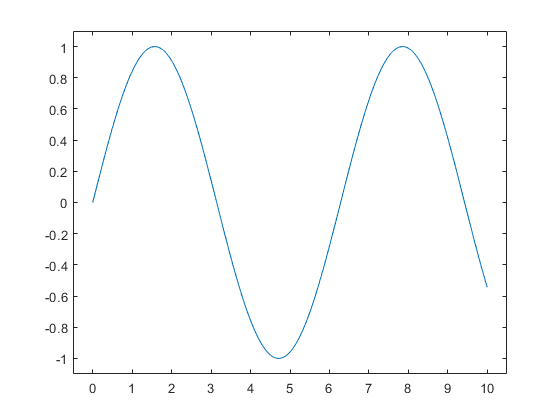
\includegraphics{images/plot_simple.png}

\hypertarget{xyy-graph}{%
\subsubsection{XYY-Graph}\label{xyy-graph}}

Mit \texttt{yyaxis} kann die Y-Achse beim selben Plot mit \texttt{left}
\& \texttt{right} gewechselt werden.

\begin{Shaded}
\begin{Highlighting}[]
\VariableTok{figure}\NormalTok{(}\FloatTok{1}\NormalTok{)}\OperatorTok{;}
\VariableTok{t} \OperatorTok{=} \FloatTok{0}\OperatorTok{:}\FloatTok{0.5}\OperatorTok{:}\FloatTok{10}\OperatorTok{;}

\VariableTok{yyaxis} \VariableTok{left}\OperatorTok{;}
\VariableTok{plot}\NormalTok{(}\VariableTok{t}\OperatorTok{,} \VariableTok{sin}\NormalTok{(}\VariableTok{t}\NormalTok{))}\OperatorTok{;}
\VariableTok{xlim}\NormalTok{([}\OperatorTok{{-}}\FloatTok{0.5} \FloatTok{10.5}\NormalTok{])}\OperatorTok{;}
\VariableTok{ylim}\NormalTok{([}\OperatorTok{{-}}\FloatTok{1.1} \FloatTok{1.1}\NormalTok{])}\OperatorTok{;}

\VariableTok{yyaxis} \VariableTok{right}\OperatorTok{;}
\VariableTok{plot}\NormalTok{(}\VariableTok{t}\OperatorTok{,} \FloatTok{20}\OperatorTok{*}\VariableTok{cos}\NormalTok{(}\VariableTok{t}\NormalTok{))}\OperatorTok{;}
\VariableTok{xlim}\NormalTok{([}\OperatorTok{{-}}\FloatTok{0.5} \FloatTok{10.5}\NormalTok{])}\OperatorTok{;}
\VariableTok{ylim}\NormalTok{([}\OperatorTok{{-}}\FloatTok{20.5} \FloatTok{20.5}\NormalTok{])}\OperatorTok{;}
\end{Highlighting}
\end{Shaded}

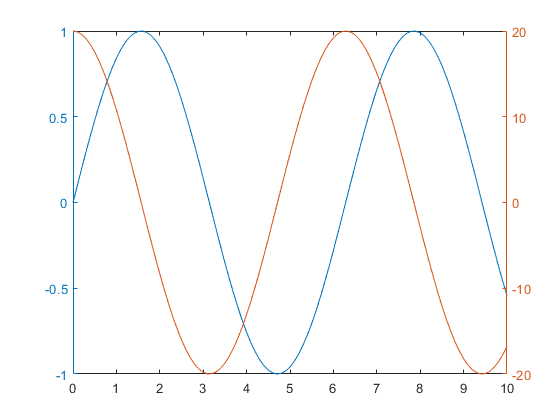
\includegraphics{images/plotyy.png}

\hypertarget{simulink}{%
\section{Simulink}\label{simulink}}

\end{multicols}

\hypertarget{glossar}{%
\section{Glossar}\label{glossar}}

\begin{itemize}
\tightlist
\item
  \emph{SISO} -- \textbf{S}ingle \textbf{I}nput \textbf{S}ingle
  \textbf{O}utput
\item
  \emph{MIMO} -- \textbf{M}ultiple \textbf{I}nput \textbf{M}ultiple
  \textbf{O}utput
\end{itemize}



\end{document}
